% updated April 2002 by Antje Endemann
% Based on CVPR 07 and LNCS, with modifications by DAF, AZ and elle, 2008 and AA, 2010, and CC, 2011; TT, 2014; AAS, 2016; AAS, 2020

\documentclass[runningheads]{llncs}
\usepackage{graphicx}
\usepackage{comment}
\usepackage{amsmath,amssymb} % define this before the line numbering.
\usepackage{color}

% INITIAL SUBMISSION - The following two lines are NOT commented
% CAMERA READY - Comment OUT the following two lines
\usepackage{ruler}
\usepackage[width=122mm,left=12mm,paperwidth=146mm,height=193mm,top=12mm,paperheight=217mm]{geometry}

\DeclareMathOperator*{\argmax}{arg\,max}
\DeclareMathOperator*{\argmin}{arg\,min}
\usepackage{mathrsfs}
\newcommand{\RED}[1]{#1}

\newcommand\TODO[1]{{\color{red}{TODO: #1}}}
\newcommand\UPDATE[1]{{\color{blue}{#1}}}
\newcommand\SOURCE[1]{{\color{green}{(from: #1)}}}


\begin{document}
% \renewcommand\thelinenumber{\color[rgb]{0.2,0.5,0.8}\normalfont\sffamily\scriptsize\arabic{linenumber}\color[rgb]{0,0,0}}
% \renewcommand\makeLineNumber {\hss\thelinenumber\ \hspace{6mm} \rlap{\hskip\textwidth\ \hspace{6.5mm}\thelinenumber}}
% \linenumbers
\pagestyle{headings}
\mainmatter
\def\ECCVSubNumber{100}  % Insert your submission number here

\title{Pixel-wise encoded patches for proposal-free instance segmentation} % Replace with your title

% INITIAL SUBMISSION 
%\begin{comment}
\titlerunning{ECCV-20 submission ID \ECCVSubNumber} 
\authorrunning{ECCV-20 submission ID \ECCVSubNumber} 
\author{Anonymous ECCV submission}
\institute{Paper ID \ECCVSubNumber}
%\end{comment}
%******************

% CAMERA READY SUBMISSION
\begin{comment}
\titlerunning{Abbreviated paper title}
% If the paper title is too long for the running head, you can set
% an abbreviated paper title here
%
\author{First Author\inst{1}\orcidID{0000-1111-2222-3333} \and
Second Author\inst{2,3}\orcidID{1111-2222-3333-4444} \and
Third Author\inst{3}\orcidID{2222--3333-4444-5555}}
%
\authorrunning{F. Author et al.}
% First names are abbreviated in the running head.
% If there are more than two authors, 'et al.' is used.
%
\institute{Princeton University, Princeton NJ 08544, USA \and
Springer Heidelberg, Tiergartenstr. 17, 69121 Heidelberg, Germany
\email{lncs@springer.com}\\
\url{http://www.springer.com/gp/computer-science/lncs} \and
ABC Institute, Rupert-Karls-University Heidelberg, Heidelberg, Germany\\
\email{\{abc,lncs\}@uni-heidelberg.de}}
\end{comment}
%******************
\maketitle


% !TEX root = ../patchEmbeddings_review.tex

\begin{abstract}
The abstract should summarize the contents of the paper. LNCS guidelines
indicate it should be at least 70 and at most 150 words. It should be set in 9-point
font size and should be inset 1.0~cm from the right and left margins.
\dots
\keywords{We would like to encourage you to list your keywords within
the abstract section}
\end{abstract}


% !TEX root = ../patchEmbeddings_review.tex

\section{Introduction}\label{sec:intro}

\emph{Instance segmentation} is a task of computer vision consisting in assigning each pixel of an image to an object instance. %, where the number of instances is usually not known in advance. 
% The most success in instance segmentation (IS) has been achieved by applying deep learning. %\cite{he2017mask,romera2016recurrent,liu2018affinity}. 
There are two main types of successful deep learning approaches to instance segmentation: proposal-based and proposal-free methods. 
Proposal-based methods consist of two steps: object detection, for example by finding bounding boxes, and assigning pixels to the detected objects. These approaches have proven to be highly successful in instance segmentation competitions like MS COCO \cite{lin2014microsoft} and CityScapes \cite{cordts2016cityscapes}. 
On the other hand, proposal-free methods adopt a bottom-up approach by directly grouping pixels into instances. Recently, there has been a growing interest for such methods that do not involve object detection, since, in certain types of images like the ones we focus on in this work, object instances cannot be approximated by bounding boxes and are usually larger than the field of view of the model.  

 
% A graph partitioning algorithm is used to obtain object instances.
Some recent successful proposal-free approaches \cite{januszewski2018high,meirovitch2016multi,liu2016multi} tackle instance segmentation by predicting, for a given patch of the input image, whether or not each pixel in the patch is part of the same instance associated to the central/anchor pixel. 
These masks are then repeatedly predicted, in a sliding window style, across the entire image and 
the final object-instances are obtained by aggregating predictions from overlapping masks.
In the following, we will refer to these patch predictions as \emph{\maskname masks}.

In this work, we propose a novel proposal-free segmentation method that is also based on the prediction of \maskname masks. However, our approach comes with the following four main advantages.
Firstly, our model concurrently predicts all \maskname masks, one for each pixel, by using a fully-convolutional approach and comes then with a much lower computational cost compared to previous patch-based methods iteratively predicting one instance at the time, one mask after the other \cite{januszewski2018high,meirovitch2016multi}.
Secondly, our approach predicts \maskname masks in a low dimensional latent representation, which allows great memory savings and let us apply the method to large volumetric images of neuron tissue \cite{arganda2015crowdsourcing}. 
Thirdly, the proposed approach aggregates predictions from overlapping \maskname masks without the need of any extra parameter or threshold;
and, finally, all final object-instances are obtained concurrently, as opposed to previous methods predicting them one-by-one with subsequent conflict resolution. 
% by extracting a set of affinities that are then used as signed weights of a graph representing the image, so that each node corresponds to a pixel

% Despite the recent successful application of patch-based methods, so far no study has been conducted to compare them with 

We also carry out a systematic study to compare the proposed model with another really common proposal-free method that has been recently successfully applied both to natural \cite{liu2018affinity,Gao_2019_ICCV} and biological \cite{lee2017superhuman,wolf2018mutex,bailoni2019generalized} images. This alternative method is sketched in Fig. \ref{fig:main_figure}a and consists of a fully-convolutional network predicting, for each pixel, a small set of short- and long-range affinities, i.e. neighborhood relations representing how likely it is for a pair of pixels to belong to the same object instance. 
\TODO{} Our comparison on neuron segmentation shows how... (equally efficient, results, etc...)


% In this work, we focus on a proposal-free method, where a Convolutional Neural Network (CNN) is trained to predict, for every pixel $i$ in the image, a patch of fixed size representing a probability mask of the instance object to which pixel $i$ belongs. The mask predicted in each patch is centered at the corresponding pixel $i$ and represents then a dense local neighborhood structure of pixel $i$. Whenever the object instance associated to pixel $i$ is bigger than the size of the patch, only a partial probability mask of the object is predicted. 
% In the following, we will call these masks as \patch or LSPM.

% [A naive way to predict one $K\times K$ \patch  for each pixel in an image would be to use a fully convolutional model with $K^2$ output channels, where each channel represents a pixel of the corresponding mask. However, this approach would not scale up well with increasing sizes $K$.]

% Our first contribution is a fully convolutional model that predicts, for every pixel $i$, a representation of the associated $i$-th self-probability mask in a lower dimensional space (see Fig. \ref{fig:main_figure}). This is possible due to the fact that, among all possible neighborhood structures represented by local self-probability masks, only few of them are associated to occurring ground truth binary masks. Thus, the information included in the predicted self-probability masks can be easily encoded in a lower dimensional latent space. 



% As a second contribution, we propose two methods for converting the predicted per-pixel self-probability masks into edge weights of a graph representing the image, so that each node corresponds to a pixel and a graph clustering algorithm is used to obtain the final instance segmentation... \TODO{Parameter-free alg. to compute edge weights; experiments; summary of sections}
% One of the two methods results in a pipeline that is as efficient as the currently winning method of the CREMI challenge \emph{(more efficient actually, because of LMC...), but achieves better accuracies and, as our results shows, outputs more consistent neighborhood structures...}.
% The second proposed method yields a parameter-free algorithm achieving competitive performances, yada yada yada... 


\begin{figure}[t]
\centering
        % \includegraphics[width=0.4\textwidth,trim=0.25in 0.25in 0.68in 0.36in,clip]{./figs/SSBM_experiments.pdf} % 0.45
        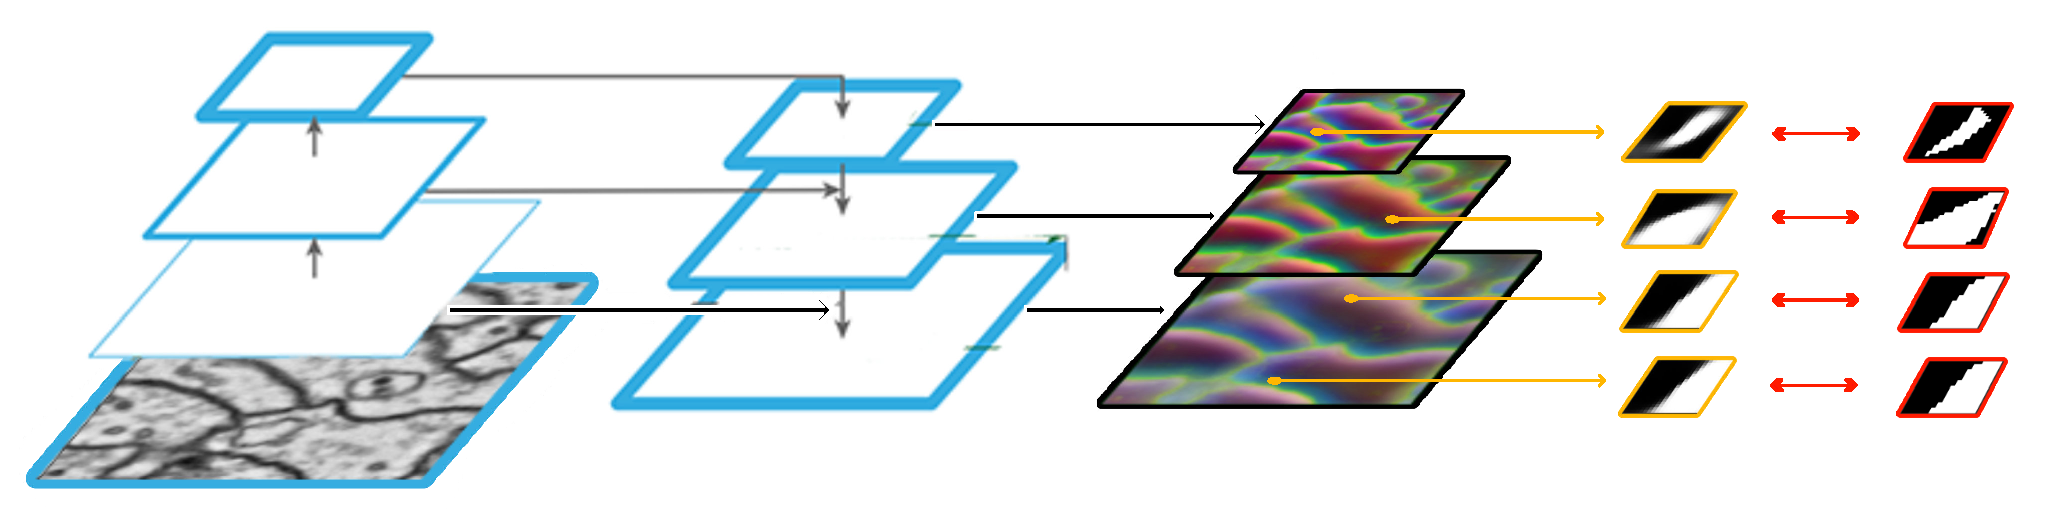
\includegraphics[width=\textwidth]{./figs/main_image.pdf} % 0.45
        \caption{A.) Predicting a sparse stencil of short- and long-range affinities. b) Predicting all patches (that it was actually the main proposal of PatchPerPix)...}
    \label{fig:main_figure}
\end{figure}




% !TEX root = ../patchEmbeddings_review.tex

\section{Related work} \label{sec:related_work}
\TODO{restructure, to be completed}

\textbf{Proposal-based methods} have been highly successful in instance segmentation competitions like MS COCO \cite{lin2014microsoft}, Pascal VOC2012 \cite{everingham2010pascal} and CityScapes \cite{cordts2016cityscapes}. They decompose the instance segmentation task into two steps that consists in generating object proposals and assigning to each bounding box a class and a binary segmentation mask \cite{he2017mask,porzi2019seamless,liu2018path,yang2012layered,li2017fully,ladicky2010and,hariharan2014simultaneous,chen2015multi,dai2016instance,liang2016reversible}. 
% They commonly rely on {Faster-RCNN}~\cite{ren2015faster} and can be trained end-to-end using non-maximum suppression. 
Other methods use instead recurrent models to sequentially generate instances one-by-one \cite{romera2016recurrent,ren2017end}.

\textbf{Proposal-free methods} adopt a bottom-up approach by directly grouping pixels into instances. Recently, there has been a growing interest for such  methods that do not involve object detection, since, in certain types of data, object instances cannot be approximated by bounding boxes. For example, the approach proposed in \cite{kirillov2017instancecut} uses a combinatorial framework for instance segmentation, 
% SGN \cite{liu2017sgn} sequentially group pixels into lines and then instances;
whereas a watershed transform is learned in \cite{bai2017deep} by also predicting its gradient direction. 
% whereas the template matching \cite{uhrig2016pixel} deploys scene depth information.
Others use metric learning to predict high-dimensional associative pixel embeddings that map pixels of the same instance close to each other, while mapping pixels belonging to different instances further apart \cite{lee2019learning,fathi2017semantic,newell2017associative,de2017semantic}. % kulikov2018instance
Final instances are then retrieved by applying a clustering algorithm, like in the end-to-end trainable mean-shift pipeline of \cite{kong2018recurrentPix}. 
Other recent successful methods simply let the model predict the relative coordinates of the instance center \cite{neven2019instance,cheng2019panopticdeeplab} or, given a point $(x,y)$ in the image, they train a model to generate the mask of the instance located at $(x,y)$ \cite{sofiiuk2019adaptis}. 

\textbf{Edge detection} also experienced recent progress thanks to deep learning, both on natural images \cite{Gao_2019_ICCV,liu2018affinity,xie2015holistically,kokkinos2015pushing} and biological data \cite{lee2017superhuman,schmidt2018cell,meirovitch2016multi,ciresan2012deep}. In neuron segmentation for connectomics, a field of neuroscience we also address in our experiments, boundaries are converted to final instances with subsequent postprocessing and superpixel-merging:
some use loopy graphs \cite{kaynig2015large,krasowski2015improving} or trees \cite{meirovitch2016multi,liu2016sshmt,liu2014modular,funke2015learning,uzunbas2016efficient} to represent the region merging hierarchy; the lifted multicut \cite{beier2017multicut} formulates the problem in a combinatorial framework, whereas 
flood-filling networks \cite{januszewski2018high} and MaskExtend \cite{meirovitch2016multi} use a CNN to iteratively grow one region/neuron at the time; recently, the work of \cite{meirovitch2019cross} made the process more efficient by employing a combinatorial encoding of the segmentation.
A structured learning approach was also proposed in \cite{funke2018large,turaga2009maximin}.

\TODO{}
 average linkage \cite{liu2018affinity,lee2017superhuman}, linkage learned by a random forest classifier \cite{nunez2013machine,knowles2016rhoananet}.


Extra approaches based signed graphs: Modern integer linear programming solvers can tackle problems of considerable size \cite{andres2012globally}, but accurate approximations \cite{pape2017solving,beier2016efficient,yarkony2012fast}, greedy agglomerative algorithms \cite{levinkov2017comparative,wolf2019mutex,keuper2015efficient,kardoostsolving} and persistence criteria \cite{lange2018partial,lange2018combinatorial} have been proposed for even larger graphs. 


proposal-free methods \cite{liu2018affinity,wolf2018mutex,lee2017superhuman} to predict long-range relationships between pixels.

\TODO{} patchPerPix, embeddings on connectomics




\clearpage
% ---- Bibliography ----
%
% BibTeX users should specify bibliography style 'splncs04'.
% References will then be sorted and formatted in the correct style.
%
\bibliographystyle{splncs04}
\bibliography{patchEmbeddings}

\end{document}
